\documentclass[a4paper]{article}

\usepackage[margin=2.5cm,headheight=50pt,includeheadfoot]{geometry}

\usepackage{amsfonts}
\usepackage{amsmath}
\usepackage{graphicx}
\usepackage{fancyhdr}
\pagestyle{fancy}
\renewcommand{\headrulewidth}{2pt}

\usepackage{xcolor}

\rhead{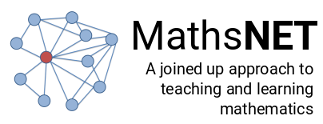
\includegraphics[width=5cm]{../../html/assets/img/logo.png}}
\lhead{\Huge SOR3012: Tutorial week 7}

\begin{document}

\section{Aim}

The aim of the tutorial this week is to look at some introductory problems on Markov chains in discrete time.

\section{Bring}

Please bring all your notes for this module as well as appropriate items of stationery.

\section{Approach}

You will work in groups of four.  Each group will try to work through as many of the problems below that they can for the first 20 minutes of the tutorial.  During the last 20 minutes of the tutorial 
each group will then be asked to give a two minute presentation of the solution to one of the problems using the visualizer.  You will be told at the start of the tutorial what problem you are 
presenting.  Remember, as you are presenting you should try to write out your solution neatly so that the other students can read what you have done.

\subsection{Question 1}

Consider the sequence of
bases/nucleotides/letters of a strand of DNA (T, A, C, G) to be the states,
$ X \in \{0,1,2,3\} $ respectively, of a
Markov chain.
The letters are abbreviations for
Thymine, Adenine, Cytosine and Guanine.
Suppose the chain is  described by the transition matrix:
$$
\left(
\begin{matrix}
0.2 & 0.3 & 0.3 & 0.2 \\
0.2 & 0.3 & 0.3 & 0.2 \\
0.2 & 0.3 & 0.2 & 0.3 \\
0.2 & 0.2 & 0.3 & 0.3 \\
\end{matrix}
\right)
$$
Calculate the probability of the following sequences:
AGT,  GTCC,   CGGT.
You may assume the first letter in the sequence  is  given (has probability 1).

\subsection{Question 2}

Consider a Markov chain with two states $X  \in  \{0, 1\}$. The  transition matrix has the form:
$$
P=
\left(
\begin{matrix}
\frac{1}{3}  &  \ \ & \frac{2}{3} \\
             &  & \\
\frac{1}{2}  & \ \ &  \frac{1}{2} \\
\end{matrix}
\right) \qquad .
$$
Calculate the following transition probabilities:
$$
P (X_1 = 1  |X_0 = 0) \qquad P (X_2 = 0|X_0 = 1) \qquad P (X_3 = 0 |X_0 = 0)
$$

\subsection{Question 3}

Consider a Markov chain between two states, $X=0$ and $X=1$,  for which
the transition matrix is given by:
$$
P=
\left(
\begin{matrix}
0.2 & 0.8 \\
0.6 & 0.4 \\
\end{matrix}
\right) \qquad .
$$
Draw the transition diagram (graph) for this chain and then calculate the following
transition probabilities:
$$
P(X_{1}=0 \vert X_{0}=0) \quad , \quad
P(X_{2}=0 \vert X_{0}=1) \quad , \quad
P(X_{3}=1 \vert X_{1}=1) \qquad .
$$
Lastly, given that $X_{0}=0$, calculate the probability of the chain (sequence) $00101$ for $X_0,X_{1},X_{2},X_{3},X_{4}$,

\subsection{Question 4}

Suppose the autumn weather in Belfast, from day to day, follows a Markov
process. If it is raining here today, there is a probability 0.3 that it
will rain again tomorrow. Similarly, the probabilities of cloudy  weather
(with no rain) or sunshine the next day are 0.5 and 0.2, respectively.
We can summarize all the transition probabilities between the states (that
is the weather from one day to the next)
$X \in \{ R,C,S \}$, in the transition matrix:
$$
P= \left(
\begin{matrix}
0.3  &   0.5  &  0.2 \\
0.3  &   0.4  &  0.3 \\
0.2  &   0.5  &  0.3 \\
\end{matrix}
\right)
\qquad .
$$
Today is a Friday in Belfast,   in  mid-October,  and it is raining.   Use the information above
to calculate the probability that both the next two days, Saturday and Sunday, will be sunny and to calculate
the probability of rain on Sunday.  Can you suggest one (or more) aspects of this model that is
unrealistic and how we might thus improve the model?

\subsection{Question 5}



Marital status for a man in his 30s is considered using the following  Markov
process. The state space of the process consists of three states: Single  ($X=0$), Cohabiting
 ($X=1$), Married  ($X=2$).

The transition matrix  from  year to year has the following form:
$$
P=
\left(
\begin{matrix}
 0.60  &   0.35  &  0.05  \\
 0.20  &   0.70  &  0.10  \\
 0.10  &    0.05 &  0.85
\end{matrix}
\right) \qquad .
$$
Draw the transition graph for this Markov chain and then answer the following questions:

\begin{itemize}
\item[(a)] Calculate the probability that a 35-year-old married man gets divorced next year, and marries again the following year.
\item[(b)] Given a 30-year-old  man is single   this year, calculate the the probability that he will still  be single in two years time.
\item[(c)] Do you think this is a good model for the marital status of a man?  What is good/bad about it? 
\end{itemize}




\end{document}
